\documentclass[10pt,a4paper]{book}
\usepackage{amsmath}
\usepackage{amsfonts}
\usepackage{amssymb}
\usepackage[english]{babel}
\usepackage{float}
\usepackage[left=2cm,right=2cm,top=2cm,bottom=2cm]{geometry}
\usepackage{graphicx}
\usepackage{hyperref} % Used for external links
\usepackage[utf8]{inputenc}
\usepackage{listings} % Used for source code listing
\usepackage{mathtools}

% Source code listing's parameters
\lstset{
  frame=single,
  keepspaces=true,
%  title=\lstname
}

\title{Second SPICE Exercise\\{\small{Fundamentals Of Electronics - a.a. 2018-2019 -
University of Padua (Italy)}}}
\author{Pietro Prandini (mat. 1097752)}

\begin{document}
\maketitle

\vspace*{\fill}
% License
\begin{center}
\tiny{This work is licensed under the Creative Commons Attribution-ShareAlike 4.0 International License. To view a copy of this license, visit \href{http://creativecommons.org/licenses/by-sa/4.0/}{http://creativecommons.org/licenses/by-sa/4.0/} or send a letter to Creative Commons, PO Box 1866, Mountain View, CA 94042, USA.}
\end{center}

\tableofcontents

\chapter{Analytic solution}

\begin{figure}[h]
  \centering
  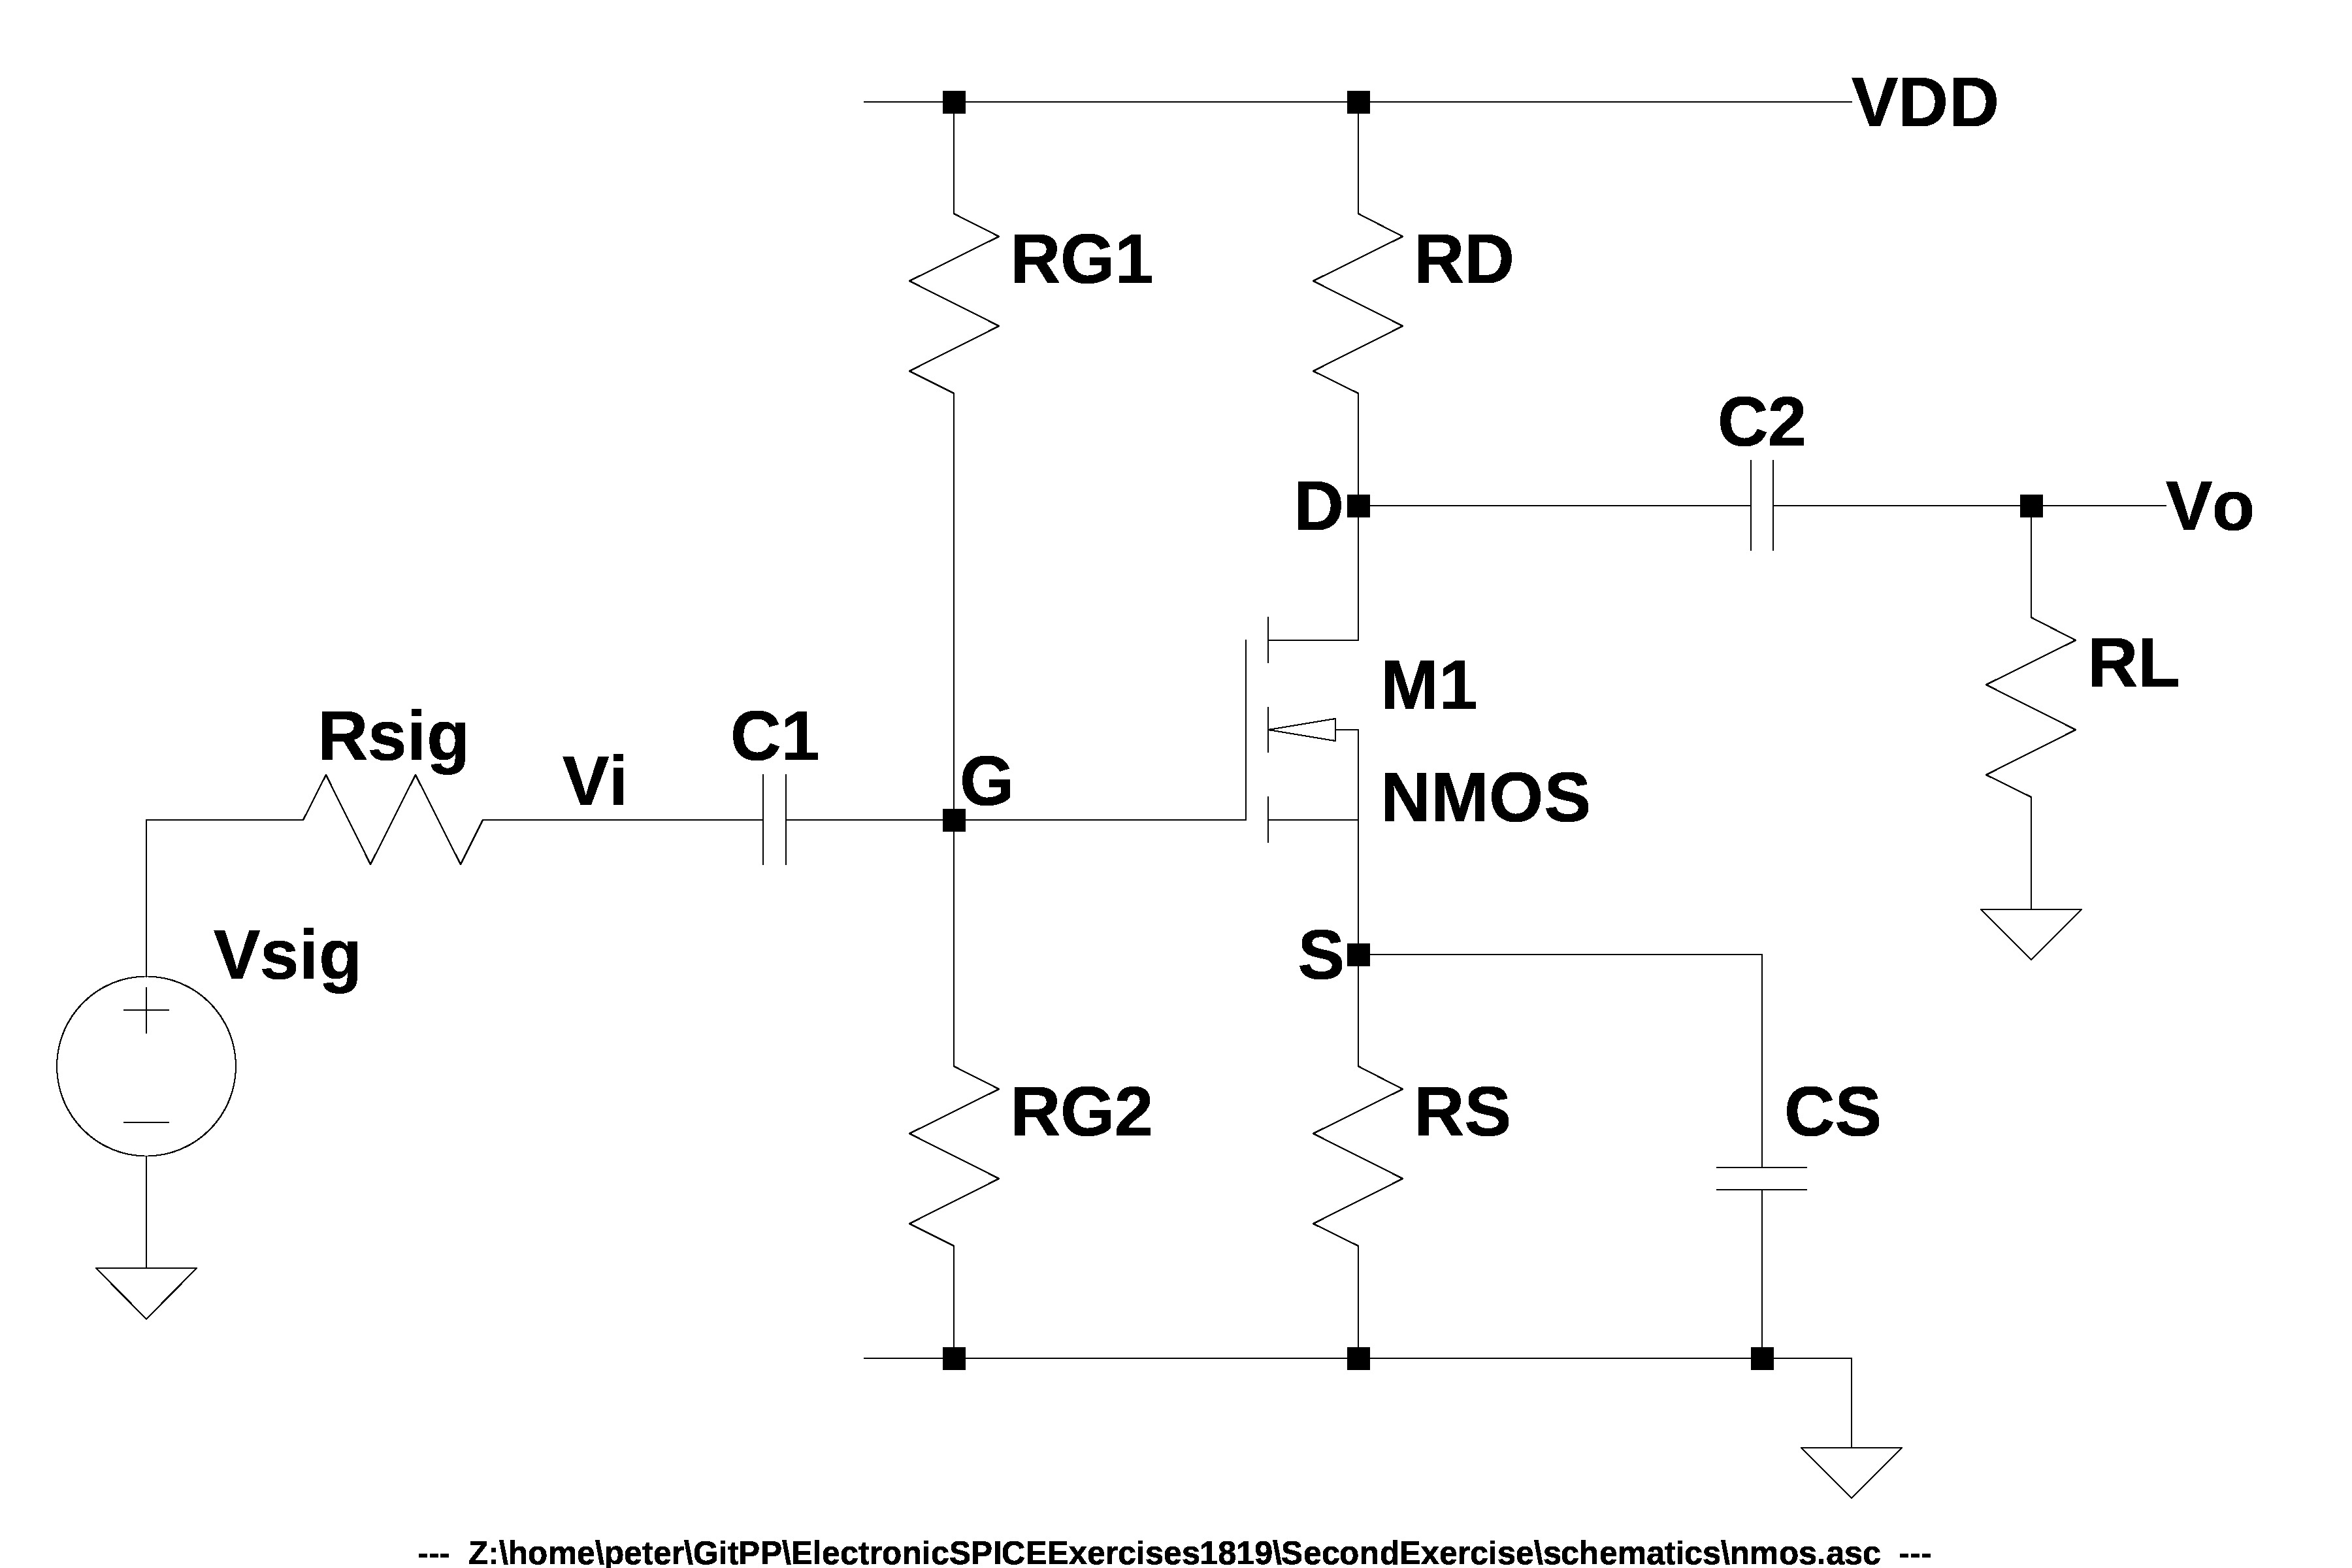
\includegraphics[width=12cm]{schematics/nmos.jpg}
  \caption{NMOS common source amplifier}
  \label{nmos}
\end{figure}

Designing the common source amplifier of the figure \ref{nmos} .\\
The MOSFET should have a $V_t = 1V$, a $K_n = 4mA/V$ and a $\lambda = 0$.\\
Other requested parameters are: $I_{DQ} = 0.5mA$, $V_S = 3.5V$, $V_D = 11V$, $V_{DD} = 15V$ and $R_{G2} = 1097752\Omega$.\par

\section{Designing by a DC analysis}
On a Direct Current analysis the capacitances can be considered as open circuits, the inductances can be considered as short circuits, the signal and the load are removed and the alternate inputs are not considered.\\
The figure \ref{nmos_DC} represents the circuit for the DC analysis.\par

\begin{figure}[h]
  \centering
  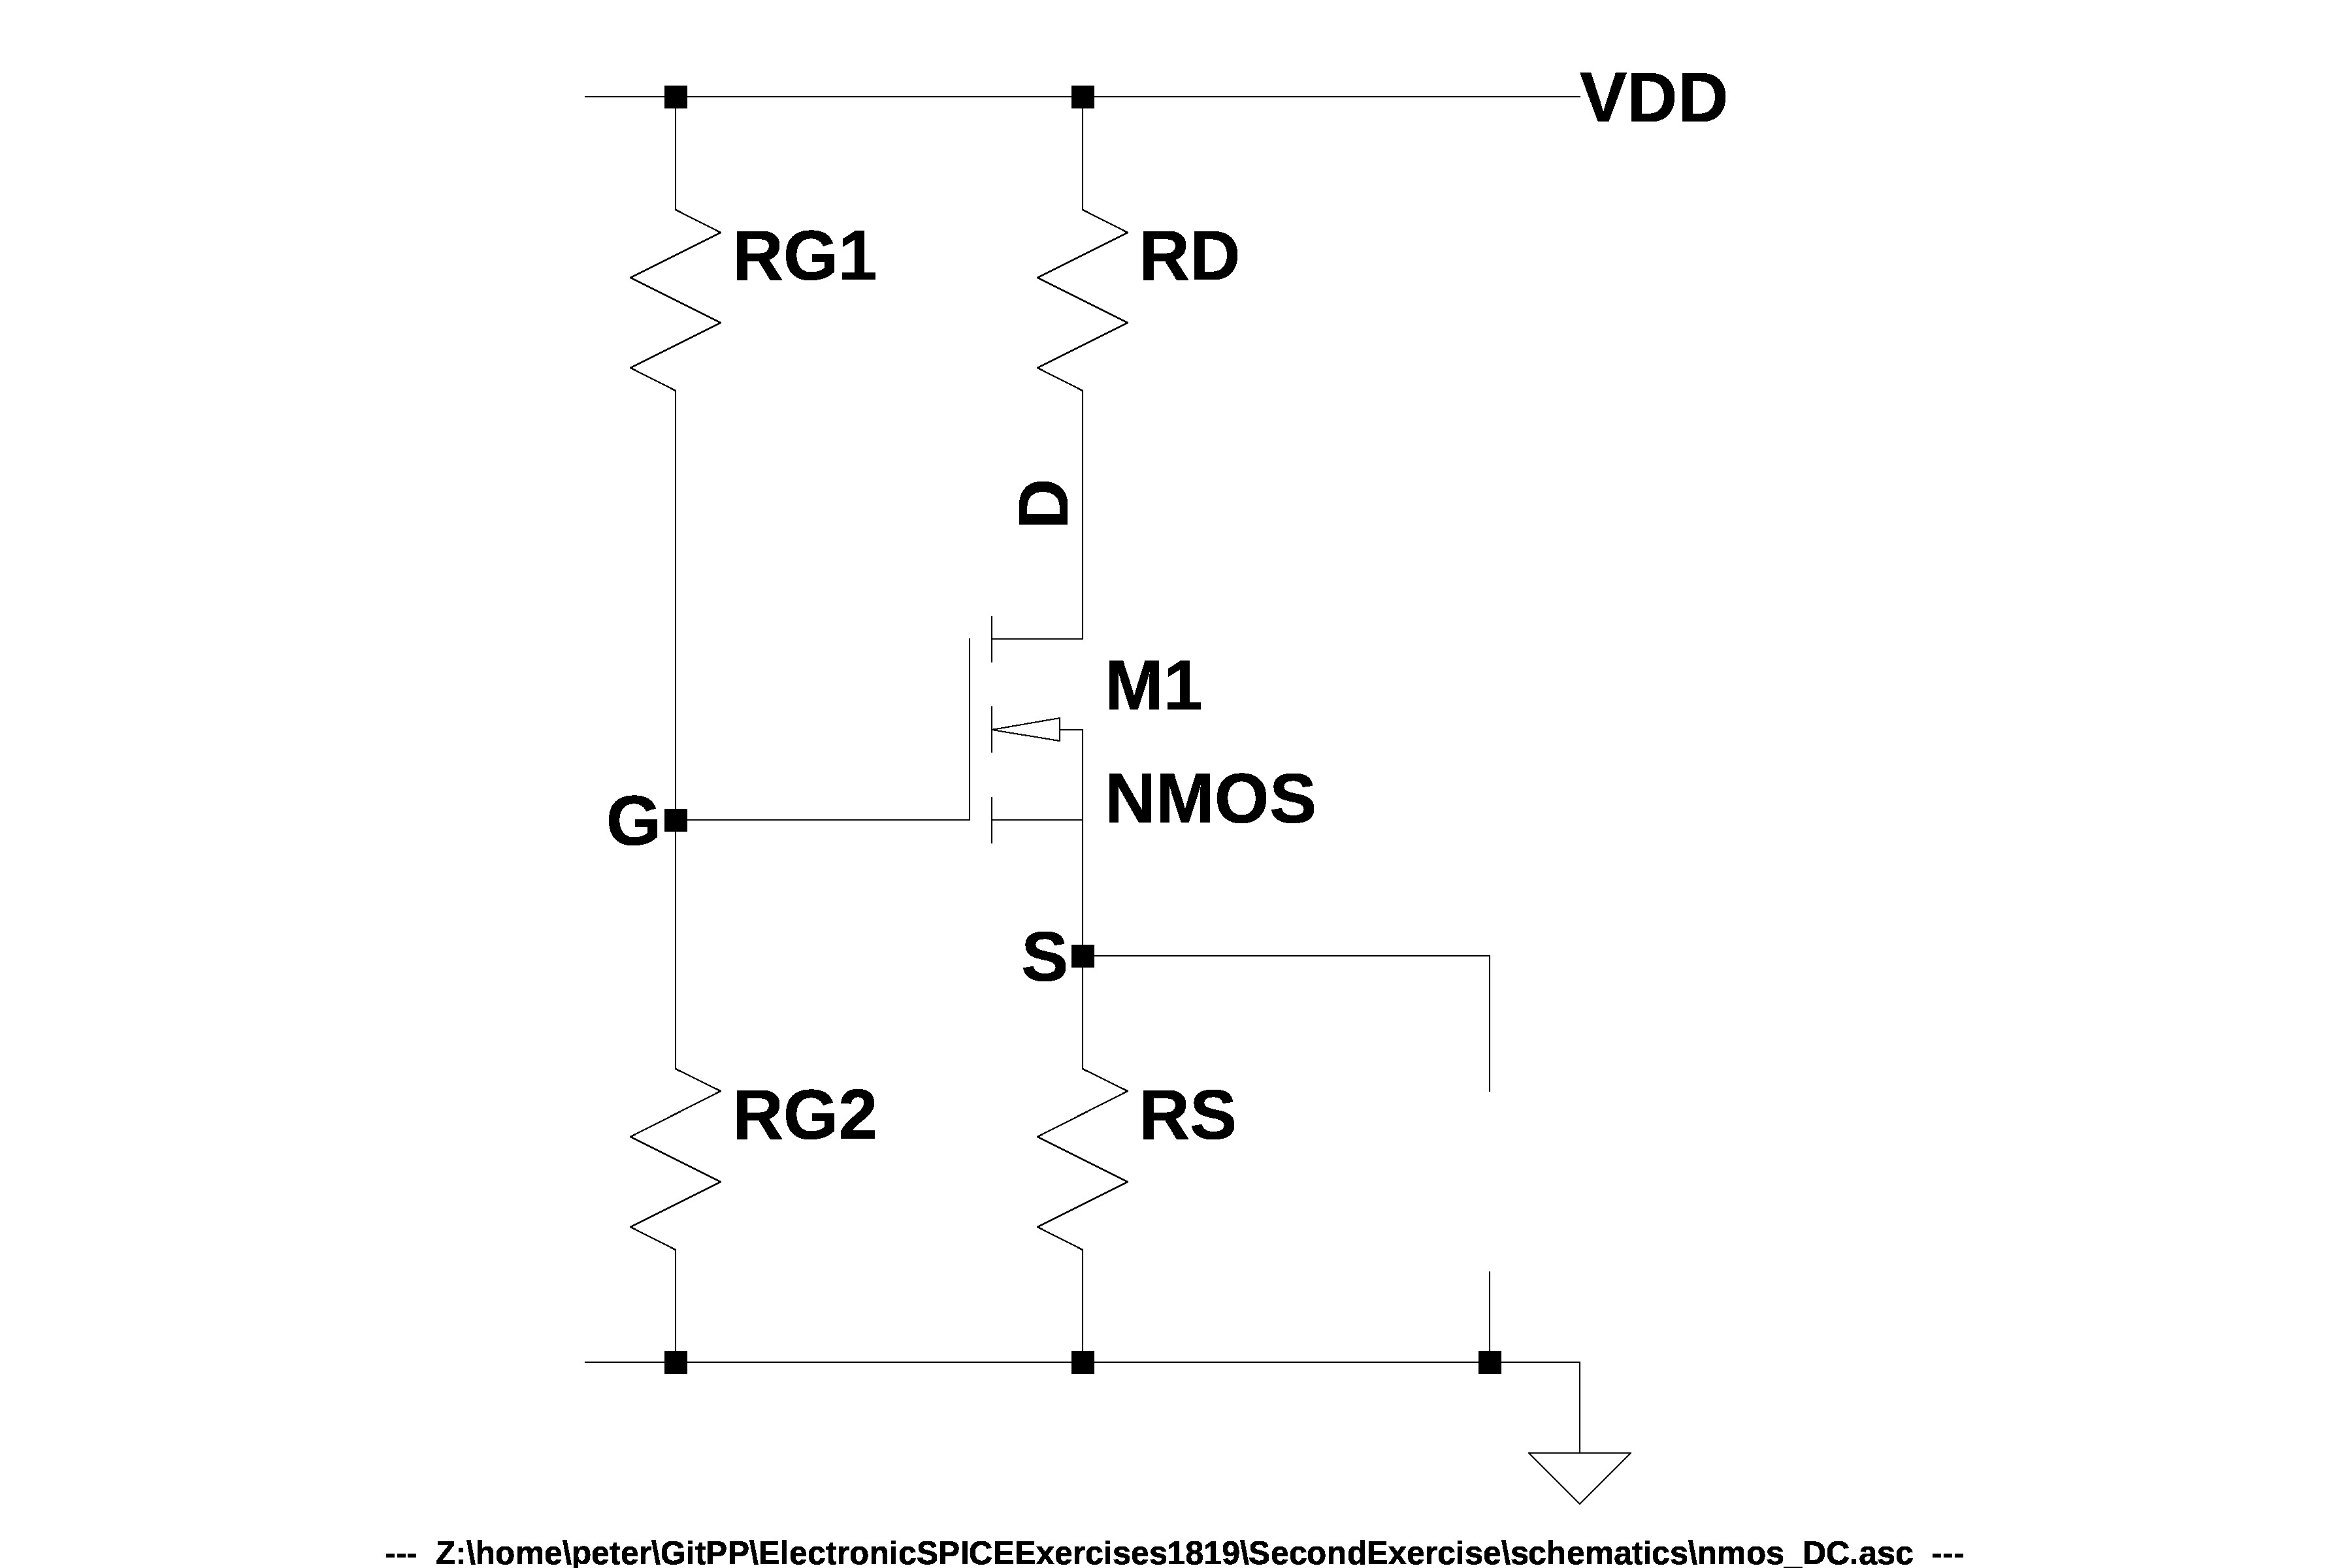
\includegraphics[width=12cm]{schematics/nmos_DC.jpg}
  \caption{NMOS common source amplifier - DC analysis}
  \label{nmos_DC}
\end{figure}

\subsection{$R_D$}
\begin{align}
V_{D} &= V_{DD} - R_D I_D\\
R_D &= \frac{V_{DD} - V_D}{I_D}\\
R_D &= \frac{15V - 11V}{0.5mA} = 8k\Omega
\end{align}

\subsection{$R_S$}
\begin{align}
V_S = R_S I_D \implies 
R_S = \frac{V_S}{I_D}\\
R_S = \frac{3.5V}{0.5mA} = 7k\Omega
\end{align}

\subsection{$V_{GS}$}
\begin{align}
I_D = \frac{1}{2}K_nV_{ov}^2 \implies
V_{ov} = \pm \sqrt{\frac{2 I_D}{K_n}}\\
V_{ov} = \pm \sqrt{\frac{2 \cdot 0.5mA}{4 mA/V^2}}\\
V_{ov} =
\left\{\begin{array}{l}
  + 0.5V \quad \text{Real value of } V_{ov} \text{.}\\
  - 0.5V \quad \text{No physical sense.}\\
\end{array}\right.\\
\end{align}
\begin{align}
V_{ov} = V_{GS} - V_{t} \implies
V_{GS} = V_{ov} + V_{t}\\
V_{GS} = 0.5V + 1V = 1.5V\\
\end{align}

\subsection{$R_{G1}$}
\begin{align}
V_{GS} = V_G - V_S \implies
V_G = V_{GS} + V_S\\
V_G = 1.5V + 3.5V = 5V\\
\end{align}

\begin{align}
I_G R_{G2} - V_{GS} - I_D R_S = 0 \implies
I_G = \frac{V_{GS}+I_D R_S}{R_{G2}}\\
I_G = \frac{1.5V + 0.5mA \cdot 7k\Omega}{1097.752k\Omega} = 4.5547628\mu A \simeq 4.55 \mu A\\
\end{align}

\begin{align}
R_{G1} &= \frac{V_{DD} - V_G}{I_G}\\
&= \frac{15V - 5V}{4.5547628 \mu A}\\
&=2.19550 M\Omega \simeq 2.20 M\Omega
\end{align}

\subsection{$g_m$}
\begin{align}
g_m = K_n V_{ov} = 4 mA/V^2 \cdot 0.5V = 2 mA/V
\end{align}

\subsection{$r_0$}
\begin{gather}
r_0 = \frac{1}{\lambda I_D} \xRightarrow{\lambda = 0} r_0 = \infty  \quad r_0 \text{ is considered an open circuit.}\\
\end{gather}

\begin{figure}[h]
  \centering
  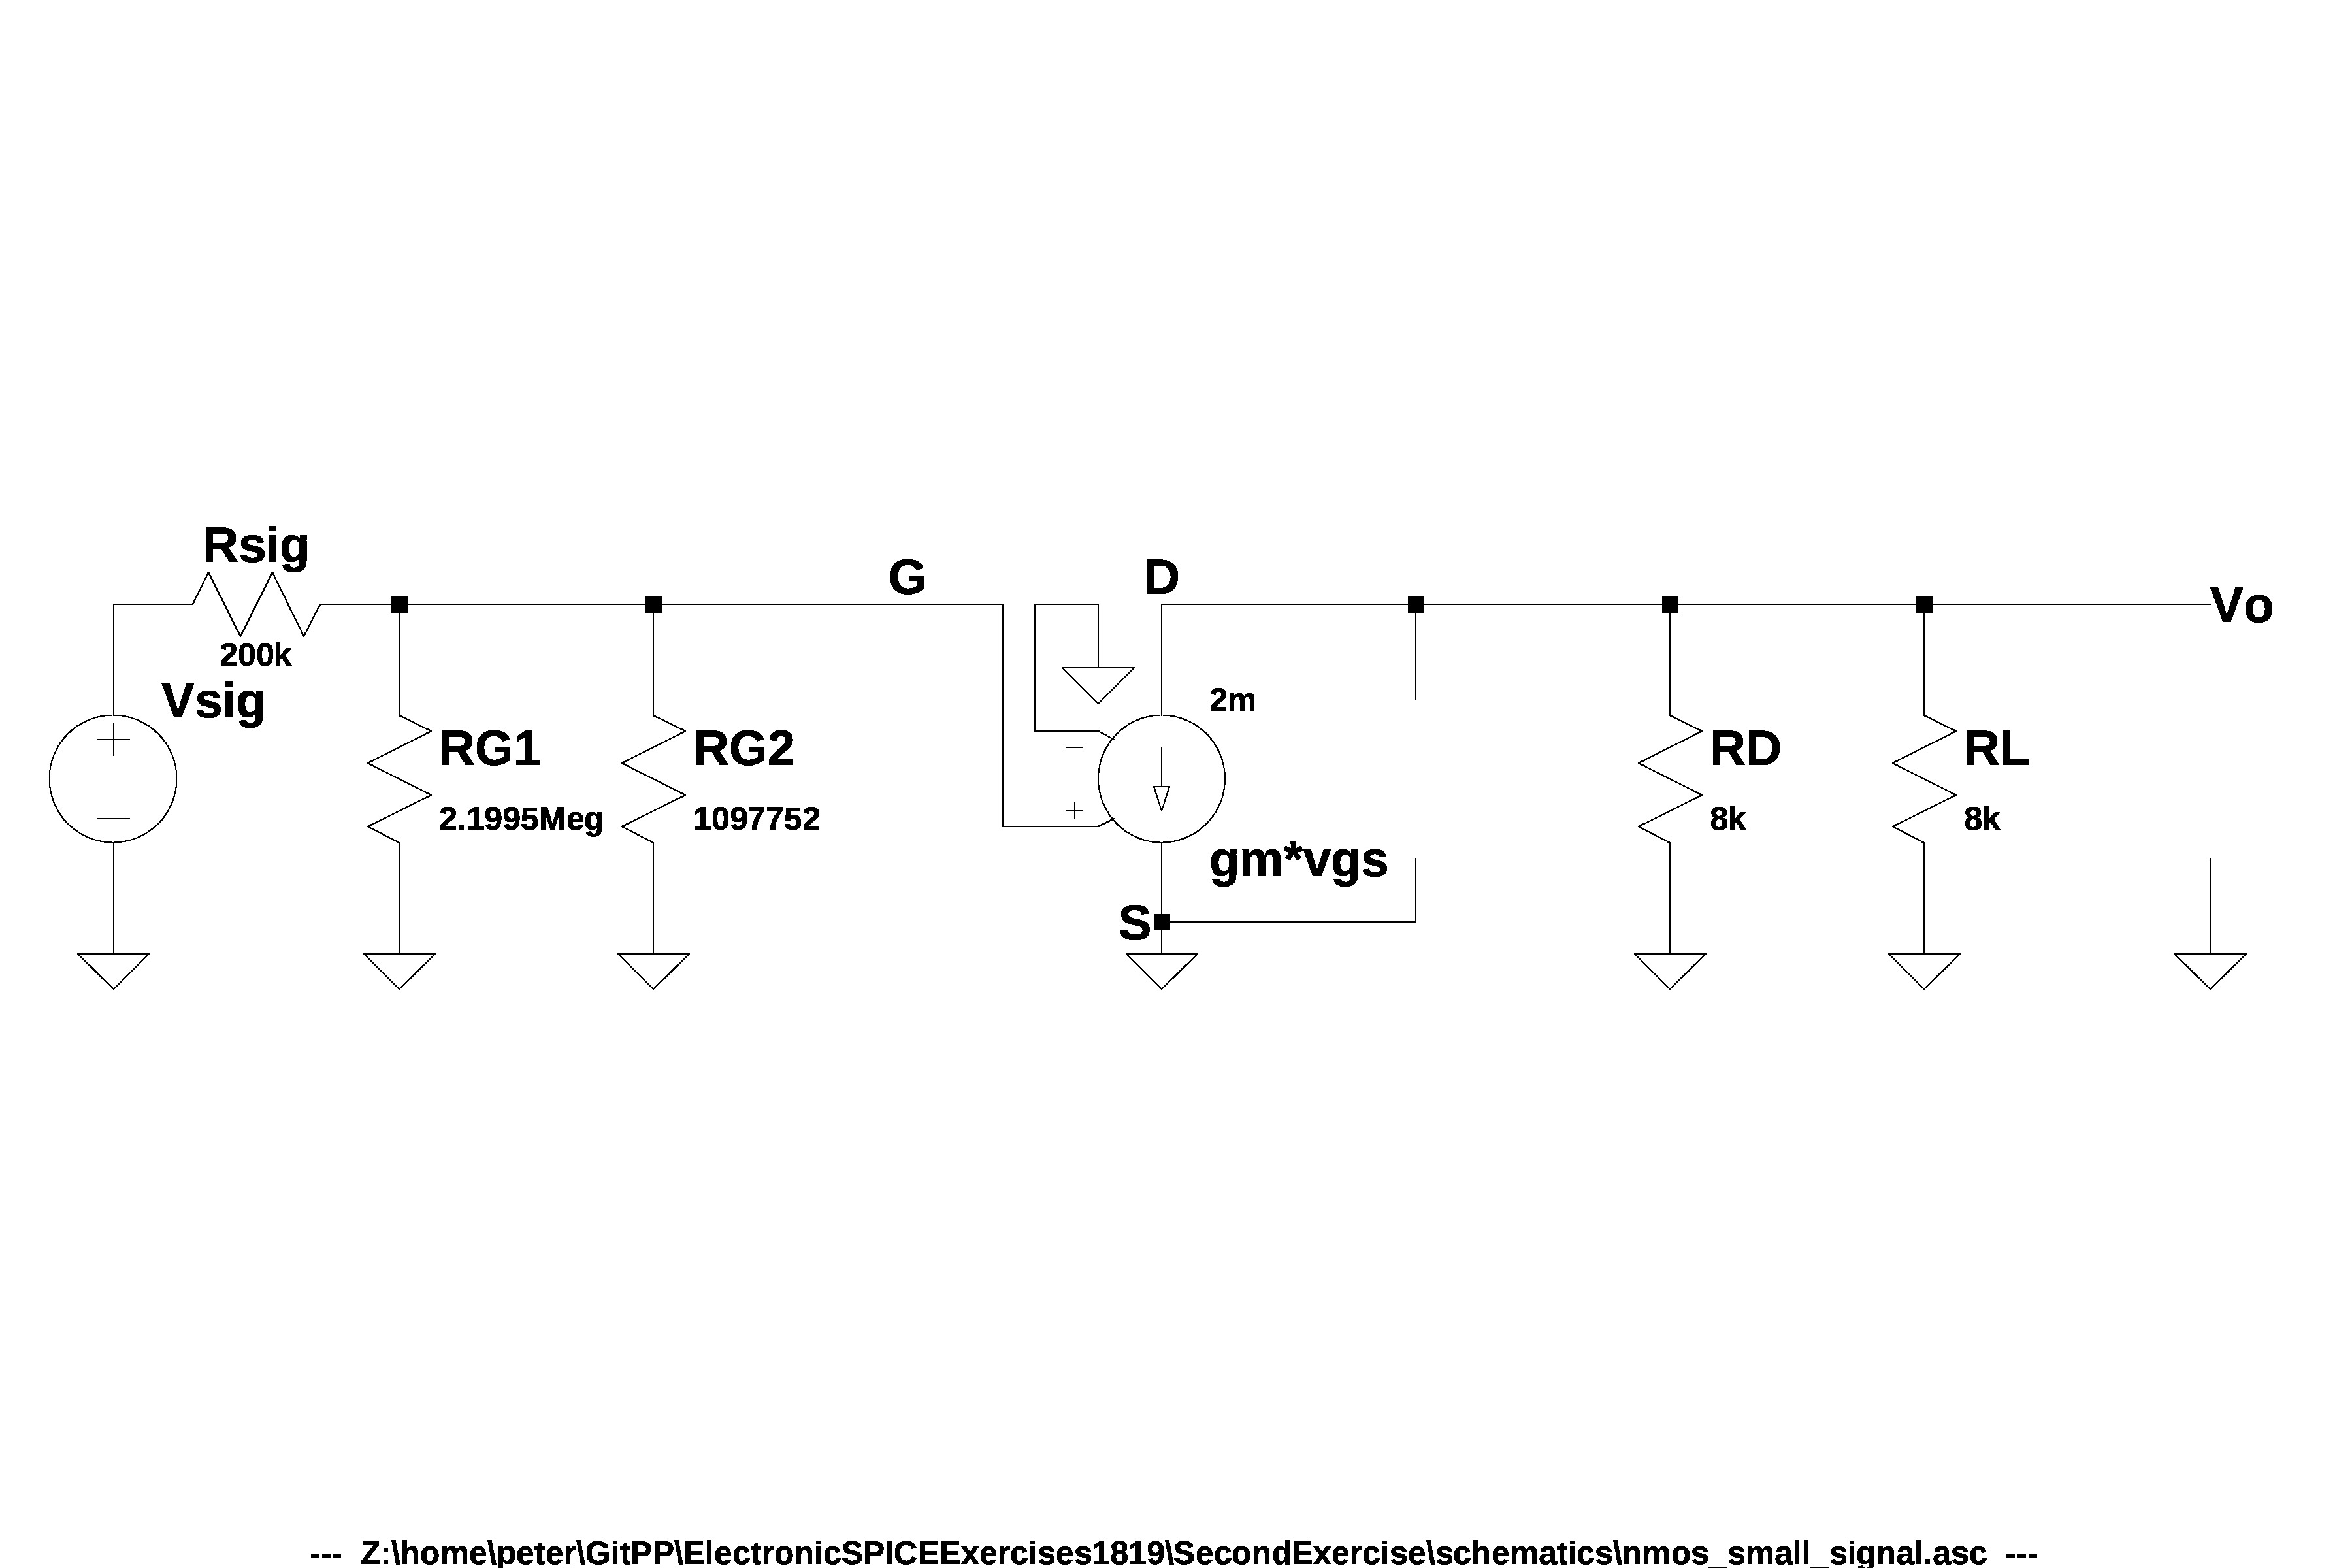
\includegraphics[width=12cm]{schematics/nmos_small_signal.jpg}
  \caption{NMOS common source amplifier - AC analysis}
  \label{nmos_AC}
\end{figure}


\chapter{SPICE simulations}

\end{document}
